\chapter{Molecular electrostatic potentials in complex space}
\label{chap:complex-space-potentials}



As we have seen in chapters \ref{chap:R-matrix} and \ref{chap:multi-channel}, the $R$-matrix correlation-driven yield can be written down as \eqref{e3-correlation-driven-yield-reprise-with-full-derivatives}, which is essentially of the form
\begin{align}
a_{nm}^{(1)}(\vb{p},\tn)
& =
-i
e^{-iE_n \tn}
e^{iI_{p,m} \ts+\frac{i}{2} \int_T^{\ts}\left(\vbp+\vba(\tau)\right)^2\d\tau} 
\int_{\ts}^T\!
e^{+i(E_n-E_m)t''}
\Vnm{\rl(t'')}
R_m(\vbp)
\d t''
\label{e4-correlation-driven-yield-recap}
\end{align}
if we ignore for the moment our hard-won corrections from chapter~\ref{chap:multi-channel} (which are nevertheless of an equivalent form) as well as the Coulomb corrections of chapter~\ref{chap:R-matrix}. From this expression we know essentially everything we need to get some hard numbers, except for the correlation interaction potential
\begin{equation}
\Vnm{\vbr}=\matrixel**{n}{\sum_{j=1}^{N-1} \frac{1-\delta_{nm}}{\| \vbr - \hat{\vbr}_j\|} }{m}
.
\label{e4-correlation-interaction-potential-initial}
\end{equation}
The purpose of this chapter is to examine this potential as a function of $\vbr$. 

This is in principle rather straightforward, as it is only the expectation value of a Coulomb kernel -- a bread-and-butter component of quantum chemistry -- but as we have seen before, we need to query this potential at the laser-driven trajectory
\begin{equation}
\rl(t) = \int_{\ts}^{t} \left[ \vbp+\vba(\tau) \right] \: \d\tau,
\end{equation}
and in general this is complex: the ionization time $\ts$ from \eqref{e2-ts-equation} is complex, so the integration variable $\tau$ must be complex, and this forces the analytical vector potential $\vba(\tau)=-\frac{F}{\omega}\ue_{z} \sin(\omega \tau)$ to also be complex. In chapter~\ref{chap:quantum-orbits} we will explore the structure of this complex-valued trajectory -- how complex it can be, how that interacts with the correlation interaction potential and the mean-field Coulomb potential, and to what extent the imaginary parts of $\rl(t)$ can be kept to a minimum -- but, for the moment, this chapter simply accepts that $\Vnm{\vbr}$ needs to be queried at complex-valued arguments, and studies the consequences.


We will find that for several common models of the orbitals that generate $\Vnm{\vbr}$, including models general enough to generate the state of the art numerical calculations for the orbitals, the corresponding analytical continuations for $\Vnm{\vbr}$ can agree surprisingly well (when $\vbr$ is `real~enough'), but they can also differ catastrophically (when $\vbr$ is `too~imaginary'), or even be impossible to generalize into a correct analytical continuation. 

The result is a serious constraint on the positions at which we can reliably calculate $\Vnm{\vbr}$ (and indeed even know what behaviour to expect), and a strong argument can be made that we completely lack the tools to venture further. On the other side, this limit also increases our confidence in $\Vnm{\vbr}$ in the regions where we \textit{can} calculate it, and, moreover, it gives us a clear goal to address in chapter~\ref{chap:quantum-orbits}, where we will show that it is indeed possible to steer the complex trajectory $\rl(t'')$ so that we never need to query $\Vnm{\rl(t'')}$ at the positions where the numerical methods fail and the analytical models disagree.



\section{Quantum chemical calculations of correlation interaction potentials for real positions}

For a real argument $\vbr$, the correlation interaction potential in \eqref{e4-correlation-interaction-potential-initial} is actually rather straightforward to calculate, since it is just the matrix element of a function of the $\vbr_j$ between two well-defined ionic eigenstates. As such, one can simply insert a position-space resolution of the identity,
\begin{equation}
1
=
\int\!\d\vbr_1\cdots\d\vbr_{N-1} \:
\ket{\vbr_1,\ldots,\vbr_{N-1}}\bra{\vbr_1,\ldots,\vbr_{N-1}}
,
\end{equation}
to rephrase the potential as an $(N-1)$-dimensional integral:
\begin{equation}
\Vnm{\vbr}
=
\sum_{j=1}^{N-1} 
\int\!
\frac{
  \braket{n}{\vbr_1,\ldots,\vbr_{N-1}} \!
  \braket{\vbr_1,\ldots,\vbr_{N-1}}{m}
  }{
  \| \vbr - \vbr_j\|
  }
\d\vbr_1\cdots\d\vbr_{N-1} 
.
\label{e4-correlation-interaction-potential-integral}
\end{equation}
(For convenience, we forget the factor of $\delta_{mn}$, which requires us to remember to impose $n\neq m$ on all uses of $\Vnm{\vbr}$.)

In general, for real $\vbr$, these are are well-behaved integrals. They have integrable square-root singularities at $\vbr_j=\vbr$, where the Coulomb kernel is multiplied by the transition charge density $ \braket{n}{\vbr_1,\ldots,\vbr_{N-1}} \!  \braket{\vbr_1,\ldots,\vbr_{N-1}}{m}$ (which is in principle complex-valued), and these are in generally smooth and rather well-behaved, with support confined to rather small regions around the molecule.


We can get a lot of intuition about the correlation interaction potentials of the form \eqref{e4-correlation-interaction-potential-integral} by working in the simplest Hartree-Fock regime, in which the ground state
\begin{equation}
\ket{\Psi_g} = \mathbb{A}\ket{\phi_1}\otimes \cdots\otimes \ket{\phi_N}
\end{equation}
is a minimal Hartree-Fock determinant, a single antisymmetrized product of single-particle orbitals $\ket{\phi_j}$, and the ionic eigenstates can be approximated well by simply deleting the relevant orbitals from the ground state. In this case the correlation interaction potential simplifies to a one-particle integral of the form
\begin{equation}
\Vnm{\vbr}
=
\sum_{j=1}^{N-1} 
\int\!
\frac{
  \phi_n^*(\vbr')\phi_m(\vbr')
  }{
  \| \vbr - \vbr'\|
  }
\d\vbr'
\label{e4-correlation-interaction-potential-hartree-fock}
\end{equation}
or, in terms of a transition charge $\rho_{mn}(\vbr') = \phi_n^*(\vbr') \phi_m(\vbr')$, as 
\begin{equation}
\Vnm{\vbr}
=
\int\!
\frac{
  \rho_{mn}(\vbr')
  }{
  \| \vbr - \vbr'\|
  }
\d\vbr'
.
\label{e4-correlation-interaction-potential-with-transition-charge}
\end{equation}
For rigorous calculations, one should of course use the fullest form available, but the Hartree-Fock intuition is useful in predicting the overall behaviour of $\Vnm{\vbr}$. For example, this form justifies our use of a dipole model for the $\X\to\B$ transition in $\mathrm{CO}_2$ in chapter~\ref{chap:multi-channel}.


Similarly, the full-form potential \eqref{e4-correlation-interaction-potential-integral} can also be written down in the single-particle integral form \eqref{e4-correlation-interaction-potential-with-transition-charge} by using the slightly more complicated transition charge density
\begin{align}
\rho_{mn}(\vbr')
 =
(N-1)
\int\!
\d\vbr_2 \cdots \d\vbr_{N-1} 
&   
\braket{n}{\vbr',\vbr_2,\ldots,\vbr_{N-1}} \!
%\nonumber \\ & \qquad \times
\braket{\vbr',\vbr_2,\ldots,\vbr_{N-1}}{m}
,
\label{e4-full-transition-charge-as-integral}
\end{align}
which encapsulates the $\vbr$-independent integration over all the other electrons.

Either way, the correlation interaction potential can always be written down in the form \eqref{e4-correlation-interaction-potential-with-transition-charge}, as a simple single three-dimensional integral of some transition charge $\rho_{mn}(\vbr')$ times a standard, perfectly integrable Coulomb kernel. As such, the correlation interaction potential can be thought of as the electrostatic field that would be produced by a charge density $\rho_{mn}(\vbr')$, complex-valued as it might be.



In practice, unfortunately, obtaining exact analytical expressions for $\Vnm{\vbr}$ for realistic cases is impossible, starting with the fact that there are no molecules for which we know exact analytical solutions for the electronic eigenstates. In fact, even for the simplest known molecular system, the hydrogen molecular ion H$_2^+$, with only a single electron responding to two clamped nuclei, the single-dimensional Schrödinger equation is separable but not exactly solvable. Similarly, as soon as there is more than one electron present -- starting with atomic helium -- exact analytical solutions of the Schrödinger equation simply do not exist.

The response to this over the past eight decades has been to develop numerical methods to solve the Schrödinger equation to as good a precision as one can reasonably ask for, by using some suitable discretization of the available state space and then numerically solving a finite-dimensional eigenvalue problem, and this is the core of the discipline of quantum chemistry. 

Within this discipline, the prevailing methods to discretize the state space for the electron wavefunctions involve the postulation of some finite basis of single-electron functions,
\begin{equation}
B=\left\{\chi_1,\ldots,\chi_M\right\},
\end{equation}
possibly optimized for the problem at hand in some variational way, and then working with $n$-electron wavefunctions built as linear combinations of Slater determinants of those basis functions. In general, these basis functions are mostly chosen to be so-called Slater-type orbitals of the form $e^{-r/\alpha}$, depending exponentially on the distance $r$ to some fixed point in space, or even more commonly gaussian-type orbitals of the form $e^{-r^2/\sigma^2}$, both of which can be modified by polynomial factors to give them better angular momentum properties.

In the end, though, what matters for our purposes is that the transition charge density $\rho_{mn}(\vbr')$, when calculated through quantum chemical means, will typically be completely constrained to be finite linear combinations of gaussian densities centred at some arbitrary location in the molecule, possibly multiplied by some polynomial. This then allows us to replace the arbitrary-looking $\rho_{mn}(\vbr')$ by a fixed gaussian charge density
\begin{equation}
\rhog(\vbr')=\normg \exp(-r'^2/\sigma^2)
\label{e4-gaussian-charge-density}
\end{equation}
if it is necessary to build intuition for the behaviour of the potential \eqref{e4-correlation-interaction-potential-with-transition-charge} when it is calculated via quantum chemical means, in the informal understanding that the full quantum chemical transition charge density is a linear superposition of such densities or polynomially related ones, and therefore so will the potential, which depends linearly on $\rho_{mn}(\vbr')$.


Here it is important to note that the gaussian potential \eqref{e4-gaussian-charge-density} is not quite a perfect model for a transition charge of the form \eqref{e4-full-transition-charge-as-integral}, because transition charges must always integrate to zero:
\begin{align}
\int \!
\rho_{mn}(\vbr')
\, \d\vbr'
& =
(N-1)
\int\!
\d\vbr' \,
\d\vbr_2 \cdots \d\vbr_{N-1} 
\braket{n}{\vbr',\vbr_2,\ldots,\vbr_{N-1}} \!
\braket{\vbr',\vbr_2,\ldots,\vbr_{N-1}}{m}
\nonumber \\ & =
\braket{n}{m}
= 0
.
\end{align}
In terms of simplified models, the gaussian potential \eqref{e4-gaussian-charge-density} can easily be modified to have this property, with the simplest and most physically relevant example being a $p$-type gaussian of the form $\rho_{\mathrm{g}, z} (\vbr')=z'\rhog(\vbr')$. The results in this chapter are essentially unchanged with this modification (which is most easily seen by noting that $\rho_{\mathrm{g}, z} (\vbr')$ is the derivative of $\rhog(\vbr')$ with respect to shifts in the origin), though the loss of rotational symmetry makes the analysis more awkward.

Similarly, when quantum chemists use simple gaussians as a basis to represent a transition charge, the nature of the coefficients is always such that, although each term, as in \eqref{e4-gaussian-charge-density} or multiplied by a polynomial, will have a nonzero charge, all these charges must add to zero.



\section{Quantum chemical potentials for complex positions}
\label{sec:quantum-chemical-potentials-complex}
Somewhat more practically, even for simple gaussian charge densities of the form \eqref{e4-gaussian-charge-density}, it is often cheap enough to simply perform the integral \eqref{e4-correlation-interaction-potential-with-transition-charge} for $\Vnm{\vbr}$ numerically, since it is relatively well behaved (its integrable singularity aside) and can be computed relatively quickly. For a quantum chemical transition charge density, known numerically in terms of the eigenfunctions of a finite-dimensional problem, this certainly seems to be a rather reasonable route, and for real positions it tends to work well.


What we want, of course, is to extend \eqref{e4-correlation-interaction-potential-with-transition-charge} to complex positions, but at least as a first stab it is reasonable to simply put in a complex-valued $\vbr$ and churn away at the numerical integral. In this case, then the integral is of the form
\begin{align}
\Vnm{\vphantom{\sum} \Re(\vbr)+i\Im(\vbr)}
& =
\int\!
\frac{
  \rho_{mn}(\vbr')
  \: \d\vbr'
  }{
  \sqrt{ \left( \Re(\vbr)+i\Im(\vbr) - \vbr' \right)^2 }
  }
\nonumber \\ & =
\int\!
\frac{
  \rho_{mn}(\vbr')
  \: \d\vbr'
  }{
  \sqrt{ \left( \Re(\vbr)-\vbr' \right)^2 - \Im(\vbr)^2 + 2i\Im(\vbr)\cdot (\Re(\vbr)-\vbr')}
  }
,
\label{e4-correlation-interaction-potential-with-complex-position}
\end{align}
which is not all that problematic, at least at first glance.

There is, for sure, the issue of exactly what branch to take for the square root, but unless there are strong over-riding reasons this is settled by the fact that -- absent knowledge of $\vbr$ and the support through $\rho_{mn}(\vbr')$ for the $\vbr'$ that are relevant to the integral -- the argument of the square root is in general conjugate-symmetric with respect to inversion in $\vbr'$ (i.e. inverting $\vbr'$ roughly conjugates the square root argument), and this generally requests that the square root be taken in a conjugate-symmetric way. This requires, then, that we define the square root with a branch cut on the ray $(-\infty,0]$, so
\begin{equation}
\sqrt{\zeta}=\sqrt{|\zeta|e^{i\theta}} = |\zeta|^{1/2} e^{i\theta/2}
\label{e4-square-root-definition}
\end{equation}
whenever the argument $\zeta$ is written as $\zeta=|\zeta|e^{i\theta}$ for $-\pi< \theta \leq \pi$. Throughout this work we will adhere strictly to this convention for the symbol $\sqrt{\phantom{zz}}$ unless otherwise noted.


\begin{subequations}
In addition to this, the change from real to complex $\vbr$ does change the structure of the integrand, by changing the nature of the singularity in the denominator. More concretely, having a vanishing denominator now requires a \textit{pair} of conditions,
\begin{align}
\left( \Re(\vbr)-\vbr' \right)^2 & = \Im(\vbr)^2 \quad \text{and} \\
 (\vbr'-\Re(\vbr)) \cdot \Im(\vbr) & =0,
\end{align}
and this changes the dimensionality of the singularity from a point to (in general) a non-degenerate line. This singularity is now the intersection of a plane through the $\Re(\vbr)$ orthogonal to $\Im(\vbr)$ and a sphere of radius $\|\Im(\vbr)\|$ around $\Re(\vbr)$, and this means that whenever $\Im(\vbr)\neq 0$ it is always a circle of radius $\|\Im(\vbr)\|$ centred at $\Re(\vbr)$, on a plane orthogonal to $\Im(\vbr)$.
\label{e4-circular-singularity}%
\end{subequations}%

Here the added dimension does make the singularity less noble -- there's ``more singularity'' to handle -- but it is still perfectly manageable, since locally at the singularity it looks mostly like a straight line, so it is of the form
\begin{equation}
\int_\mathrm{local}  \frac{\d x'\d y'\d z'}{\sqrt{(x'-x_0)^2+(y'-y_0)^2}}
\end{equation}
(i.e. with the $z$ dimension regularized out, but still a line singularity at $x'=x_0$, $y'=y_0$), and this is still regular when the area element in the $x',y'$ plane $\d x'\d y'=r'\d r'\d\theta'$ is taken into account. Of course, if the integration is done numerically the ring singularity must still be specifically handled to obtain correct results, but it does not represent a significant impediment to the calculation.


\captionsetup[figure]{position=top}
\begin{figure}[htb]
  \centering
  \begin{tabular}{cc}
  \subfloat[$\Re(\Vg(\vbr))$]{
    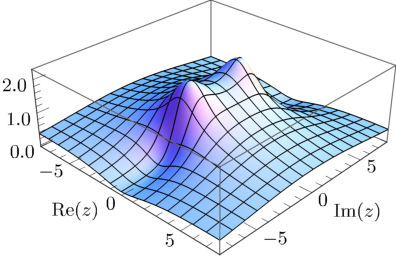
\includegraphics[scale=1]{4-Potentials/Figures/figure4Aa.pdf}
  }
  &
  \subfloat[$\Im(\Vg(\vbr))$]{
    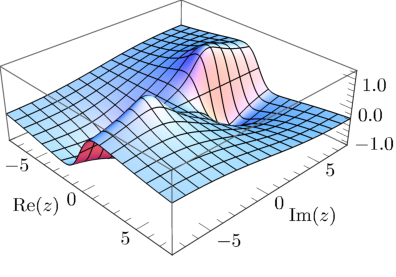
\includegraphics[scale=1]{4-Potentials/Figures/figure4Ab.pdf}
  }
  \end{tabular}
  \caption[Numerically integrated electrostatic potential $\Vg(\vbr)$ of a gaussian charge distribution as a function of complex space coordinates]{
  Electrostatic potential $\Vg(\vbr)$ of a gaussian charge distribution as a function of complex $z$ for fixed $x=3$ and $y=0$, with $\sigma=1$, calculated using direct numerical integration as in \eqref{e4-correlation-interaction-potential-numerically-gaussian}.}
  \label{f4-numerical-potential-from-gaussian}
\end{figure}
\captionsetup[figure]{position=auto}


With all this in hand, then, we can now simply plug in a complex position into \eqref{e4-correlation-interaction-potential-with-complex-position}, do the integral numerically, and see what comes out. As a starting example, to keep things simple, we can use a single gaussian charge distribution at the origin, $\rhog(\vbr)$ as in \eqref{e4-gaussian-charge-density}, so we look to calculate
\begin{align}
\Vg\left(\vphantom{\sum} \Re(\vbr)+i\Im(\vbr)\right)
& =
\int\!
\frac{
  \normg \exp(-r'^2/\sigma^2)
  \: \d\vbr'
  }{
  \sqrt{ \left( \Re(\vbr)-\vbr' \right)^2 - \Im(\vbr)^2 + 2i\Im(\vbr)\cdot (\Re(\vbr)-\vbr')}
  }
.
\label{e4-correlation-interaction-potential-numerically-gaussian}
\end{align}
This single integral can readily be integrated numerically, and we show the results in \reffig{f4-numerical-potential-from-gaussian}, fixing two components of $\vbr$ and showing the variation of $\Re(\Vg(\vbr))$ and $\Im(\Vg(\vbr))$ as a function of complex $z$ while keeping $x$ and $y$ constant. (Because of the rotational symmetry of $\rhog(\vbr)$, of course, these results are essentially representative, up to the shape parameter $\sqrt{x^2+y^2}/\sigma$.)




This procedure, then, gives us a very workable electrostatic potential: it is continuous, with no poles, branch points, or other singularities, and it is bounded at infinity. More physically, it contains two large bumps when $z=i\zeta$ is imaginary and of the same magnitude as $|x|$ because then the quadratic term $\Re(\vbr^2)=x^2-\zeta^2$ in
\begin{align}
\Vg(x,0,i\zeta)
& =
\int\!
\frac{
  \normg \exp(-r'^2/\sigma^2)
  \: \d\vbr'
  }{
  \sqrt{r'^2-2(xx'+i\zeta z')+(x^2-\zeta^2)}
  }
,
\end{align}
which effectively acts as softening, vanishes, and this leaves the Coulomb kernel at maximal amplitude. Moreover, the potential appears to be smooth and, if everything went right, it should be analytic.





Unfortunately, this combination of features turns out to be too good for our electrostatic potential, because it makes it run afoul of one of the basic principles of complex analysis: the fact that if a function is continuous and differentiable everywhere, then either it diverges to infinity or it is absolutely constant.





\pagebreak

\begin{mathaside}{Any bounded entire function is constant}
\label{aside.entire-functions-bounded}


To be more precise, a function $f:\mathbb{C} \to \mathbb{C}$ is called \textit{analytic} at $z$ if its complex derivative $f'(z)$, in the sense of the Cauchy-Riemann equations, exists at $z$ and at all points in an open neighbourhood of $z$, and it is called \textit{entire} if it is analytic (and therefore continuous) at all points $z\in\mathbb{C}$. Similarly, $f$ is bounded in a region $D$ if there exists $M>0$ such that $|f(z)|<M$ for all $z\in D$. With this language, then, we have the simple theorem:

\begin{namedtheorem}[Liouville's]
If $f:\mathbb{C} \to \mathbb{C}$ is entire and bounded for all values of $z$ in the complex plane, then $f(z)$ is constant.
\end{namedtheorem}


For a rigorous proof, we refer the reader to \citer{churchill_complex_variables}. Nevertheless, given the rather far-reaching consequences of this principle, it is worth spending some time to justify it. In its essence, Liouville's theorem is deeply related to yet another core fact of complex analysis, the maximum principle:

\begin{theorem}[Maximum principle]
If $f:U\subseteq \mathbb{C}\to\mathbb{C}$ is analytic and not constant in the interior of a region, then $|f(z)|$ has no maximum value in that interior.
\end{theorem}


Both of these statements punch far above their weight in terms of the strength of their consequences versus the simplicity of their statements, but the main ingredient here is simply the fact that both the real and imaginary parts of $f$ are harmonic functions. Indeed, if we write $f(x+iy)=u(x,y)+v(x,y)$ in terms of real-valued $u$, $v$, $x$ and $y$, then the Cauchy-Riemann equations
\begin{subequations}
\begin{empheq}[left={\empheqlbrace\,}]{align}
\frac{\partial u}{\partial x} & = \frac{\partial v}{\partial y} \\
\frac{\partial u}{\partial y} & = -\frac{\partial v}{\partial x} 
\end{empheq}
\label{e4-cauchy-riemann}
\end{subequations}
imply that both $u$ and $v$ obey the Laplace equation,
\begin{equation}
\frac{\partial^2 u}{\partial x^2}+\frac{\partial^2 u}{\partial y^2}
=
\frac{\partial^2 v}{\partial x^2} + \frac{\partial^2 v}{\partial y^2}
= 0
.
\end{equation}
Thus, if they are `winding down', with convex curvature, in one dimension, they must be `winding up' with concave curvature in the orthogonal dimension. This means that both $u$ and $v$ must obey the maximum principle -- no harmonic function can sustain a local maximum in the interior of its domain -- and, after some technical wrangling with the Cauchy-Riemann equations to extend the argument to $|f(z)|=\sqrt{u^2+v^2}$, so does $f$.
\qed

\vspace{\maskip}

At this level, we can already see that the numerical $\Vg(\vbr)$ shown in \ref{f4-numerical-potential-from-gaussian} simply has no chance of being an analytical function, since both its real and imaginary parts are obviously not harmonic functions, and they both show obvious local maxima and minima.


Liouville's theorem follows much of the same intuition -- if a function is entire, then it must keep growing for bigger and bigger circles -- but it requires an independent proof. More specifically, we take some arbitrary $z_0\in \mathbb{C}$, and we relate the value of the derivative $f'(z_0)$ there to the values of $f(z)$ on some arbitrary circle $C$ about $z_0$ of radius $r$ using Cauchy's integral formula,
\begin{equation}
f'(z_0) = \frac{1}{2\pi i}\int_C \frac{f(z)\d z}{(z-z_0)^{2}}
.
\end{equation}
Since we know that $|f(z)|$ is bounded everywhere by some constant $M>0$, we can take the absolute values of both sides to get an inequality
\begin{equation}
|f'(z_0)|\leq \frac{1}{2\pi} \frac{M\times 2\pi r}{r^2} = \frac{M}{r}
.
\end{equation}
Here $M$ was given and fixed, but $r$ can be chosen to be arbitrarily large, and this requires that $f'(z_0)=0$ for our arbitrary $z_0\in\mathbb{C}$; in other words, $f(z)$ is constant. 

\hfill\qedsymbol

\vspace{\maskip}
A bit away from the formal side, both of these principles express the fact that the theory of analytical functions is very, very rigid, and even more so when compared to the theory of smooth real functions in $C^\infty$. This rigidity boils down to the fact that to be complex differentiable a function $f$ must not only be locally well approximated by a straight line, as in the real case; instead, it must also obay the the full-fledged pair of Cauchy-Riemann differential equations in~\eqref{e4-cauchy-riemann}. The rigidity of the theory is, at least partly, inherited from the theory of differential equations, which is rigid enough that functions tend to inherit their values in the interior of a region from their behaviour at its boundary.

\vspace{\maskip}
On a more positive note, Liouville's theorem is best seen as the statement that for a function to be analytic, it needs to be interesting: it needs to have poles, branch cuts, natural boundaries, or divergences at infinity. Our numerically integrated $\Vg(\vbr)$ from \eqref{e4-correlation-interaction-potential-numerically-gaussian} and \reffig{f4-numerical-potential-from-gaussian}, with its gentle bumps and bounded, continuous behaviour, does not qualify.



\end{mathaside}



Returning to our numerically-integrated potential, we see that its features indicate that it cannot be an analytical function of $x$, $y$ and $z$. However, we do not need to take this for granted -- we can simply check to see whether it obeys the Cauchy-Riemann equations, which is shown in \reffig{f4-cauchy-riemann-for-numerical-gaussian}. As expected from the above considerations, of course, the test fails, which means that our numerically-integrated $\Vg(\vbr)$ is not an analytical function.



\captionsetup[figure]{position=top}
\begin{figure}[htb]
  \centering
  \begin{tabular}{cc}
  \subfloat[$\Im \left( \frac{\partial \Vg(\vbr)}{\partial \Re(z)} \right)$]{
    \label{f4-cauchy-riemann-for-numerical-gaussian-a}
    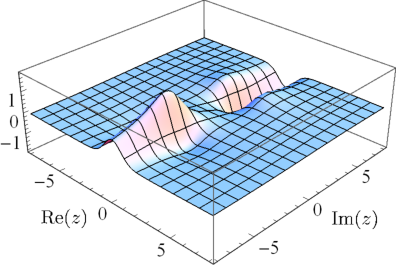
\includegraphics[scale=1]{4-Potentials/Figures/figure4Ba.pdf}
  }
  &
  \subfloat[$\Im \left( \frac{\partial \Vg(\vbr)}{i \, \partial \Im(z)} \right)$]{
    \label{f4-cauchy-riemann-for-numerical-gaussian-b}
    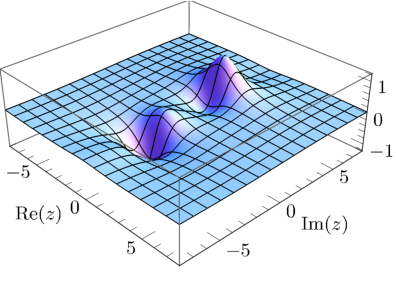
\includegraphics[scale=1]{4-Potentials/Figures/figure4Bb.pdf}
  }
  \\
  \subfloat[$\Re \left( \frac{\partial \Vg(\vbr)}{\partial \Re(z)} \right) \approx \Re\left( \frac{\partial \Vg(\vbr)}{i \, \partial \Im(z)} \right)$]{
    \label{f4-cauchy-riemann-for-numerical-gaussian-c}
    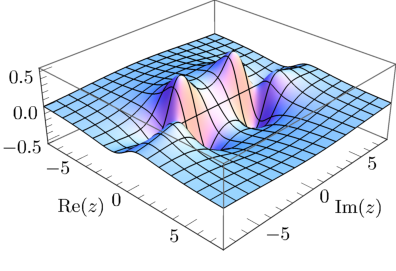
\includegraphics[scale=1]{4-Potentials/Figures/figure4Bc.pdf}
  }
  &
  \subfloat[$\left| \frac{\partial \Vg(\vbr)}{\partial \Re(z)} - \frac{\partial \Vg(\vbr)}{i \, \partial \Im(z)} \right|$]{
    \label{f4-cauchy-riemann-for-numerical-gaussian-d}
    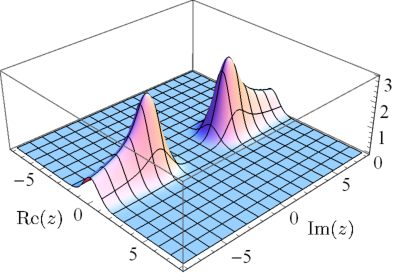
\includegraphics[scale=1]{4-Potentials/Figures/figure4Bd.pdf}
  }
  \end{tabular}
  \caption[Cauchy-Riemann equations for the numerically-integrated dlectrostatic potential $\Vg(\vbr)$ over complex coordinates]{
  Cauchy-Riemann equations for the numerically-integrated electrostatic potential $\Vg(\vbr)$ of \eqref{e4-correlation-interaction-potential-numerically-gaussian}, shown over the same slice of complex coordinate space as \reffig{f4-numerical-potential-from-gaussian} ($x=3$, $y=0$, and complex $z$).
  Panels~\protect\subref{f4-cauchy-riemann-for-numerical-gaussian-a} and~\protect\subref{f4-cauchy-riemann-for-numerical-gaussian-b} show the imaginary parts of the derivative of $\Vg(\vbr)$ with respect to the real and imaginary parts of $z$, respectively; for an analytical function they should match but instead they have immediately appreciable differences. The real parts, shown in~\protect\subref{f4-cauchy-riemann-for-numerical-gaussian-c}, do match, but the two derivatives are left with a strong difference, shown in~\protect\subref{f4-cauchy-riemann-for-numerical-gaussian-d}.
  }
  \label{f4-cauchy-riemann-for-numerical-gaussian}
\end{figure}
\captionsetup[figure]{position=auto}



The reason for why $\Vg(\vbr)$ fails to be analytical can be seen, at least after the fact, from its integral form \eqref{e4-correlation-interaction-potential-with-complex-position}. There, when we write
\begin{align}
\Vg(\vbr)
& =
\int\!
\frac{
  \normg \exp(-r'^2/\sigma^2)
  }{
  \sqrt{ \left( \vbr-\vbr' \right)^2}
  }
\d\vbr'
,
\label{e4-correlation-interaction-potential-for-analyticity}
\end{align}
we are expressing $\Vg(\vbr)$ as a continuous superposition of Coulombic point-charge potentials $1/\sqrt{ \left( \vbr-\vbr' \right)^2}$, and these are not analytic when $\vbr'$ lies in the circular singularity, as described by \eqref{e4-circular-singularity}, with respect to $\vbr$. Since the integral always includes points $\vbr'$ at this singularity and its neighbourhood, the assumption of analyticity of the resulting integral should be seen as suspect from the~start.







\section{Exactly integrable potentials}
We see, then, that the formulation of our correlation interaction potential $\Vnm{\vbr}$ as an integral over the ionic electrons' positions must be reformulated from its foundations when the probe point $\vbr$ is complex-valued. This is somewhat problematic, since we initially defined $\Vnm{\vbr}$ as the matrix element 
\begin{equation}
\Vnm{\vbr}=\matrixel**{n}{\sum_{j=1}^{N-1} \frac{1-\delta_{nm}}{\| \vbr - \hat{\vbr}_j\|} }{m}
\backtag{e4-correlation-interaction-potential-initial}
\end{equation}
at the start of this chapter, and there are few ways of evaluating such matrix elements that don't rely on an integral. 

However, a more careful analysis shows that the matrix element \eqref{e4-correlation-interaction-potential-initial} is only needed when defining $\Vnm{\vbr}$ for real-valued positions, since that is what goes into the original temporal integral for the ionization yield in \eqref{e2-correlation-driven-yield-separated} and \eqref{e2-correlation-driven-yield-with-eva-states}, and the only thing we need is the analytical continuation of this $\Vnm{\vbr}$ -- obtained by any reasonable means~-- when we shift the endpoint of the temporal integral into the complex plane to arrive at~\eqref{e2-correlation-driven-yield-semi-final}. 


This would seem to offer a very small comfort, since constructive theorems on analytical continuation are few and far between, but fortunately for us our problem has plenty of structure that we can exploit. To begin with, for many of the charge densities $\rho(\vbr)$ that we care about, including gaussian and exponential charge densities, the electrostatic potential, obtained as
\begin{align}
V(\vbr)
& =
\int\!
\frac{
  \rho(\vbr') \:\d\vbr'
  }{
  \sqrt{ \left( \vbr-\vbr' \right)^2}
  }
,
\label{e4-electrostatic-potential-as-integral}
\end{align}
can actually be integrated exactly in terms of a closed elementary expression -- and, when this is possible, the elementary expression gives an automatic analytical continuation. In fact, it isn't even necessary to do a full integration, since the integral electrostatic potential in \eqref{e4-electrostatic-potential-as-integral} can  be described equally well, for real positions, as the unique solution of the Poisson equation
\begin{equation}
\nabla^2 V(\vbr)=-4\pi \rho(\vbr)
\label{e4-poisson-equation}
\end{equation}
under $V(\vbr)\to 0$ as $|\vbr|\to\infty$. In fact, for spherically symmetric charge distributions, this reduces to a simple second-order ordinary differential equation, which is much easier to integrate, and additional angular-momentum polynomial factors can also be accommodated rather easily by suitable modifications of the spherically-symmetric case.

This means, then, that for the gaussian charge distribution \eqref{e4-gaussian-charge-density} that proved so problematic earlier we can simply write down the potential as
\begin{subequations}
\label{e4-exact-gaussian-potential}
\begin{align}
\Vg(\vbr) 
& = 
\pi^{3/2} \sigma^3 \normg \frac{ \erf(r/\alpha) }{ r }
\\ & = 
Q \frac{ \erf(r/\alpha) }{ r }
,
\end{align}
\end{subequations}%
in terms of a simple error function \citenistchap{7} and the total charge $Q$. Similarly, with the other building block of quantum chemical bases, the Slater-type orbital with an exponential charge density
\begin{equation}
\rhoe(\vbr) = \norme \exp(-r/\sigma)
,
\label{e4-exponential-charge-density}
\end{equation}
the radial Poisson equation can also be trivially solved to give the potential
\begin{subequations}
\label{e4-exact-exponential-potential}%
\begin{align}
\Ve(\vbr) 
& = 
4\pi \alpha^2 \norme \left[ - \left( 1 + \frac{2\alpha}{r} \right) e^{-r/\alpha} + \frac{2\alpha}{r} \right]
\\ & = 
 \frac{Q}{2\alpha} \left[ - \left( 1 + \frac{2\alpha}{r} \right) e^{-r/\alpha} + \frac{2\alpha}{r} \right]
.
\end{align}%
\end{subequations} %

It is important to note that both of these exact potentials were obtained by integrating Poisson's equation \eqref{e4-poisson-equation} for real coordinates, and they are only equal to the integrally-defined potential \eqref{e4-electrostatic-potential-as-integral} when $\vbr$ is real. However, both exact formulas \eqref{e4-exact-gaussian-potential} and \eqref{e4-exact-exponential-potential} \textit{must} hold for the analytical continuation of \eqref{e4-electrostatic-potential-as-integral} into complex-valued $\vbr$, because for each coordinate they coincide on the real axis, and that is sufficient to ensure the uniqueness of the analytical continuation. Since the both \eqref{e4-exact-gaussian-potential} and \eqref{e4-exact-exponential-potential} are analytic, they are \textit{the} unique extension of \eqref{e4-electrostatic-potential-as-integral} to the complex plane \cite[\S108]{churchill_complex_variables}.


\vspace{5mm}


\begin{mathaside}{Analytical continuation}
\label{aside.analytical-continuation}

At this point, it is worth spending some time emphasizing this feature of the theory of complex variables. If we are given a function $f:\mathbb{R}\to \mathbb{C}$ which is `nice enough', it is usual to speak of its analytical continuation as if this extension of $f$ to the complex plane can always be done, and can always be done uniquely. The possibility and uniqueness of analytical continuation in a multiply connected region is a complicated question, which reaches fruition in the theory of Riemann surfaces. (On the other hand, it is all too common to assume that, multivaluedness issues aside, any analytical function can always be extended as far as necessary, which need not be the case: many functions run into natural boundaries, which stop any kind of analytical continuation~\cite[p.~191]{noguchi_complex_analysis}.)

\vspace{\maskip}
In our context, it is worth emphasizing just how little is really necessary to ensure the uniqueness of an analytical continuation; the standard result \cite[given e.g. in Ref.][pp.~283ff]{churchill_complex_variables} is usually stated in the form

\begin{theorem}
A function that is analytic in a domain $D$ is uniquely determined over $D$ by its values over a subdomain, or along an arc, interior to $D$.
\end{theorem}


where the key word is the concept of a \textit{domain}, which is restricted to an open, singly connected subset $D$ of $\mathbb{C}$. However, the hypotheses for this usual statement can be softened considerably \cite[p.~95]{noguchi_complex_analysis}: the agreement over a line can be loosened to agreement over a sequence $(s_n)_{n=0}^\infty \subset D$ that converges to a point $s_n\to s\in D$, or, in other words,
%%% also http://www.unc.edu/math/Faculty/met/complex.pdf

\begin{theorem}
A function that is analytic in a domain $D$ is uniquely determined over $D$ by its values on any set $S\subset D$ which has an accumulation point in $D$.
\end{theorem}


This is, again, an expression of the rigidity of the theory of analytical functions, especially when compared to the study of continuously differentiable real functions, where no similar result is even remotely true. Complex analytical functions, being the solutions of a differential equation, are much more constrained by their values on the boundary or subparts of a domain.

\end{mathaside}




Now that we have suitable analytical continuations of at least some reasonable charge distributions, the next thing to investigate is their behaviour as functions of $\vbr$. The first thing to try is to look at their behaviour over real coordinates, and here both potentials look remarkably similar (modulo some leeway on how to relate the $1/e$ widths $\sigma$ and $\alpha$ of the two charge distributions), as shown in \reffig{f4-exact-gaussian-vs-exponential-real-coordinates}. 

\begin{figure}[htb]
  \centering
  \begin{tabular}{c}
  \subfloat{  
    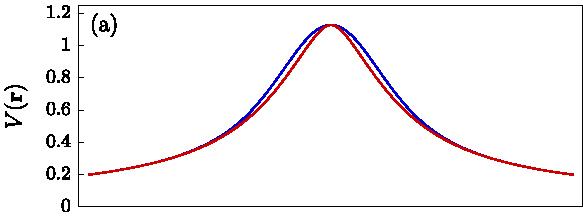
\includegraphics[scale=1]{4-Potentials/Figures/figure4Ca.pdf}
    \label{f4-potential-comparison} 
  }
  \\[-5mm]
  \subfloat{
    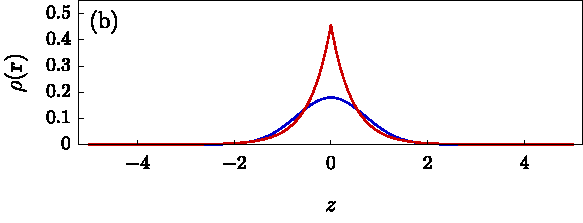
\includegraphics[scale=1]{4-Potentials/Figures/figure4Cb.pdf}
    \label{f4-charge-density-comparison} 
  }
  \end{tabular}
  \caption[Exact electrostatic potentials $\Vg(\vbr)$ and $\Ve(\vbr)$, for gaussian and exponential charge densities, over real coordinates]{
  Exact electrostatic potentials $\Vg(\vbr)$ (blue) and $\Ve(\vbr)$ (red) as a function of real coordinates, for equal total charges $Q=1$ and with the $1/e$ widths $\sigma=1$ and $\alpha=\sqrt{\pi}/4$ chosen so the potentials will match at the origin. The corresponding charge distributions are shown~in~\protect\subref{f4-charge-density-comparison}.}
  \label{f4-exact-gaussian-vs-exponential-real-coordinates}
\end{figure}


In general, gaussian distributions are rather different to Slater-type exponential orbitals, because they lack the latter's cusp at the origin, and they have markedly thinner tails at the edges. Nevertheless, if we relate the two widths by asking that the potential at the origin $V(\mathbf 0)$ be the same for both distributions, we get relatively similar charge distributions, as shown in \reffig{f4-charge-density-comparison}, and the remarkably similar electrostatic potentials of~\reffig{f4-potential-comparison}. Since the charge distributions are relatively similar blobs for both cases, we can hope that their potentials will also have similar behaviour for complex coordinates.






Unfortunately, the similarities between the two potentials end there, and when we look at their behaviour for complex coordinates we get completely different structure, shown in \reffig{f4-exact-gaussian-vs-exponential-complex-coordinates}.
% for the same cut through complex $\vbr$ space as in Figs.~\ref{f4-numerical-potential-from-gaussian} and \ref{f4-cauchy-riemann-for-numerical-gaussian} (i.e. taking a fixed $x=3$ and $y=0$ and varying $z\in\mathbb{C}$). 



\captionsetup[figure]{position=top}
\begin{figure}[htb]
  \centering
  \begin{tabular}{cc}
  \subfloat[$\Re(\Vg(\vbr))$]{
    \label{f4-re-vg-over-complex-coords}
    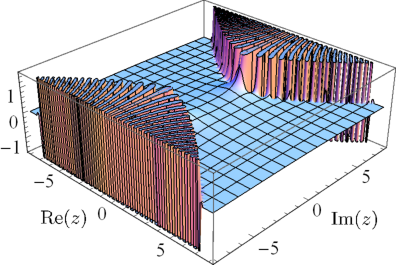
\includegraphics[scale=1]{4-Potentials/Figures/figure4Da.pdf}
  }
  &
  \subfloat[$\Im(\Vg(\vbr))$]{
    \label{f4-im-vg-over-complex-coords}
    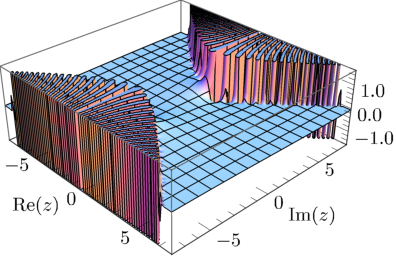
\includegraphics[scale=1]{4-Potentials/Figures/figure4Db.pdf}
  }
  \\[6mm]
  \subfloat[$\Re(\Ve(\vbr))$]{
    \label{f4-re-ve-over-complex-coords}
    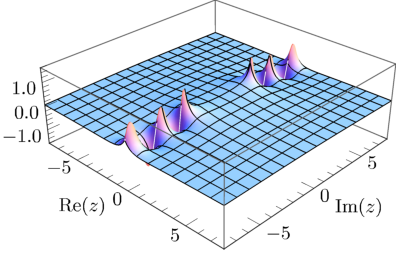
\includegraphics[scale=1]{4-Potentials/Figures/figure4Dc.pdf}
  }
  &
  \subfloat[$\Im(\Ve(\vbr))$]{
    \label{f4-im-ve-over-complex-coords}
    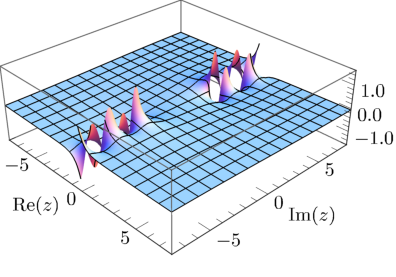
\includegraphics[scale=1]{4-Potentials/Figures/figure4Dd.pdf}
  }
  \end{tabular}
  \caption[Exact electrostatic potentials $\Vg(\vbr)$ and $\Ve(\vbr)$, for gaussian and exponential charge distributions, over complex coordinates]{
  Exact electrostatic potentials $\Vg(\vbr)$ and $\Ve(\vbr)$ over complex coordinates, with the same cut over complex space as Figs.~\ref{f4-numerical-potential-from-gaussian} and \ref{f4-cauchy-riemann-for-numerical-gaussian}. The potential $\Vg(\vbr)$ from a gaussian charge distribution diverges at imaginary coordinates, while the potential $\Ve(\vbr)$ from an exponential distribution has a branch cut there.
  }
  \label{f4-exact-gaussian-vs-exponential-complex-coordinates}
\end{figure}
\captionsetup[figure]{position=auto}


Perhaps the most salient feature of both of these potentials is the stark divergence of the exact gaussian potential $\Vg(\vbr)$ as the imaginary part of $z$ increases, which immediately becomes unmanageable regardless of the scale on the vertical axis. This can be seen quite clearly from the asymptotic expansion for the error function \citenisteq{7.12.1}, which at large and real argument describes a gaussian approach from below to 1, but inherits this $e^{-z^2}$ behaviour for the entire complex plane:
\begin{equation}
\erf(z) \sim 1 - \frac{e^{-z^2}}{\sqrt{\pi}} \left( 1- \frac{1}{z} + \frac{1}{2z^2} - \cdots \right)
\label{e4-erf-asymptotic-expansion}
\end{equation}
whenever $|\arg(z)| < \frac{3\pi}{4}$. In the potential $\Vg(\vbr)$ from \eqref{e4-exact-gaussian-potential}, the error function is called with $r=\sqrt{x^2+y^2+z^2}$ as an argument, which means that for large $|z|$ it behaves as $\exp((\Im(z)^2-\Re(z)^2)/\sigma^2)$, and if the imaginary part of $z$ is large enough then $\Vg(\vbr)$ will diverge in a super-gaussian fashion. This strong divergence is then responsible for the wall-like behaviour shown in Figs.~\ref{f4-re-vg-over-complex-coords} and \ref{f4-im-vg-over-complex-coords}. Finally, to add a slight insult to the injury, the complex exponential also oscillates ever more wildly in this region.



The potential for the exponential distribution, $\Ve(\vbr)$, on the other hand, has much more bounded behaviour, but instead of a divergence to infinity it now fills up its interestingness quota with a pair of branch cuts that stretch from $z=\pm i x$ to imaginary infinity. These branch cuts are, in fact, rather natural, because the potential is a function of $r=\sqrt{x^2+y^2+z^2}$, which itself has a sign-change branch cut when its argument is~negative. 
%%% In a sense, this branch cut is harder to deal with than the exponential divergence of $\Vg(\vbr)$, because integration contours cannot cross branch cuts


It is worth asking at this stage why the gaussian potential $\Vg(\vbr)$ does not exhibit any branch cuts on its domain: after all, it is a function of $r$ just as much as $\Ve(\vbr)$. The reason for this is that the error function is a pure odd function, and it therefore has a Taylor expansion \citenisteq{7.6.1} of the form
\begin{equation}
\erf(z)
%=\frac{2}{\sqrt{\pi}}\sum_{n=0}^{\infty} \frac{(-1)^{n}z^{2n+1}}{n!(2n+1)}
=\frac{2}{\sqrt{\pi}}\left( z - \frac{z^3}{3} + \frac{z^5}{10} - \cdots \right)
.
\end{equation}
This means, in turn, that the gaussian potential \eqref{e4-exact-gaussian-potential} also has a Taylor series of definite parity,
\begin{equation}
\Vg(\vbr) 
=
Q \frac{ \erf(r/\sigma) }{ r }
=
\frac{2Q}{\sqrt{\pi}\sigma}\left( 1 - \frac{r^2}{3\sigma^2} + \frac{r^4}{10\sigma^4} - \cdots \right)
,
\end{equation}
except that now $\Vg(\vbr)$ is a pure even function, so it is a function of $r^2$. Since $r^2$ has no branch cuts, $\Vg(\vbr)$ cannot have any either. It is this sort of subtle difference in the potentials' behaviour for real coordinates that causes the stark differences at complex coordinates shown in \reffig{f4-exact-gaussian-vs-exponential-complex-coordinates}.


The divergence in behaviour of our two potentials at complex coordinates is definitely worrisome, since they are both more or less reasonable models for real-world charge distributions. Gaussian and exponential-type orbitals are the general building blocks of quantum chemistry, and while they are certainly not interchangeable (with a definite conceptual advantage to exponential charges, since the gaussian distributions lack the cusps and long tails expected of real-world orbitals), as far as real-coordinates electrostatics is concerned they are both essentially blobs of charge that produce very similar electrostatic potentials. 


It is also important to note that this difference in behaviour is quite certain to persist through most of the common modifications to our model charge distributions. On the simplest level, the addition of polynomial factors to a gaussian charge is exactly equivalent to taking its derivatives, which means that the overall (super-)gaussian factor will always be present. A similar, more involved argument holds for exponential orbitals.

On a slightly higher level, it is also impossible to get radically different behaviour from any finite collection of gaussians, since the linearity of Poisson's equation implies that the potential will be the corresponding linear combination of $\Vg(\vbr)$'s, and it is essentially impossible for such a function to be well-behaved everywhere, since it is an entire function and we know it decays as $1/r$ or faster in all real directions, so it needs to diverge to infinity at large imaginary coordinates. 

Moreover, the behaviour at large imaginary coordinates will be dominated by the contributions from the tightest gaussians in the basis set, because these will have the shortest length scales $\sigma$, and that means that their corresponding potentials $\Vg(\vbr)\sim \exp(+\Im(\vbr)^2/\sigma^2)$ will be the fastest to explode. While there will probably be at least two of these at the same width, they are overwhelmingly unlikely to contribute in such a way that their divergences will cancel out, especially when probed over all possible lines on real space and all possible directions in the complex continuation of that real cut.  This argument, moreover, extends to transition charges that integrate to zero total charge.



Given that $\Vg(\vbr)$ and $\Ve(\vbr)$ produce wildly different potentials for complex coordinates, we are now left with the even bigger question of what should be the general features to expect of the complex-coordinates electrostatic potential $V(\vbr)$ for a realistic charge distribution -- should it have branch cuts? should it diverge exponentially? super-exponentially? should it have poles, while we're at this? -- and we are left with precious few tools to answer this question.



\captionsetup[figure]{position=top}
\begin{figure}[!htbp]
  \centering
  \begin{tabular}{cc}
  \subfloat[$\Re(\Vg(\vbr))$]{
    \label{f4-potentials-comparison-restricted-complex-coordinates-a}
    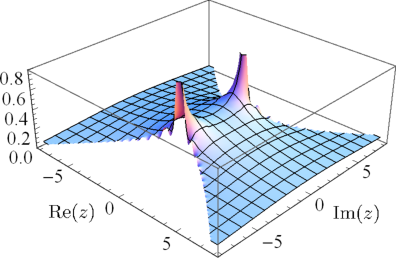
\includegraphics[scale=1]{4-Potentials/Figures/figure4Ea.pdf}
  }
  &
  \subfloat[$\Im(\Vg(\vbr))$]{
    \label{f4-potentials-comparison-restricted-complex-coordinates-b}
    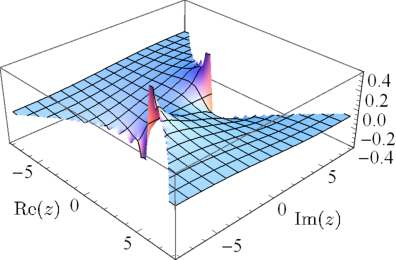
\includegraphics[scale=1]{4-Potentials/Figures/figure4Eb.pdf}
  }
  \\
  \subfloat[$\Re(\Ve(\vbr))$]{
    \label{f4-potentials-comparison-restricted-complex-coordinates-c}
    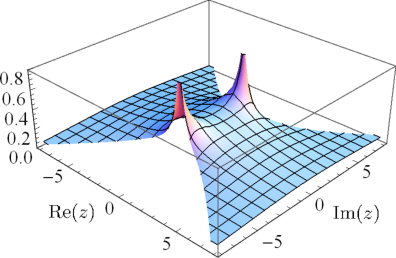
\includegraphics[scale=1]{4-Potentials/Figures/figure4Ec.pdf}
  }
  &
  \subfloat[$\Im(\Ve(\vbr))$]{
    \label{f4-potentials-comparison-restricted-complex-coordinates-d}
    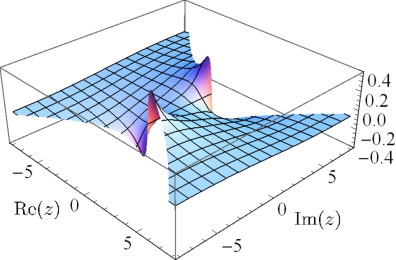
\includegraphics[scale=1]{4-Potentials/Figures/figure4Ed.pdf}
  }
  \\
  \subfloat[$\Re(\Vgnum(\vbr))$]{
    \label{f4-potentials-comparison-restricted-complex-coordinates-e}
    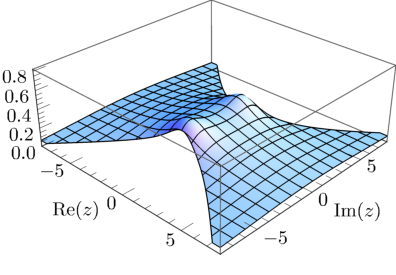
\includegraphics[scale=1]{4-Potentials/Figures/figure4Ee.pdf}
  }
  &
  \subfloat[$\Im(\Vgnum(\vbr))$]{
    \label{f4-potentials-comparison-restricted-complex-coordinates-f}
    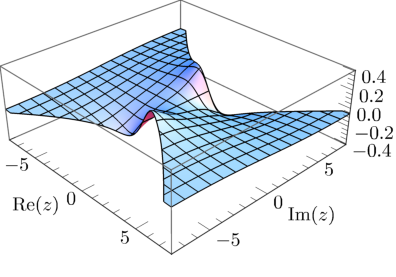
\includegraphics[scale=1]{4-Potentials/Figures/figure4Ef.pdf}
  }
  \end{tabular}
  \caption[Electrostatic potentials $\Vg(\vbr)$, $\Ve(\vbr)$ and $\Vgnum(\vbr)$ over complex coordinates restricted to $\Re(\vbr^2)>0$]{
  Exact electrostatic potentials $\Vg(\vbr)$ and $\Ve(\vbr)$ over complex coordinates (\subref*{f4-potentials-comparison-restricted-complex-coordinates-a}-\subref*{f4-potentials-comparison-restricted-complex-coordinates-d}), exactly as in \reffig{f4-exact-gaussian-vs-exponential-complex-coordinates}, but restricted to the region $\Re(\vbr^2)>0$. Despite their disagreements in coordinates that are `too imaginary' (in the sense that $\Re(\vbr^2)=\Re(\vbr)^2-\Im(\vbr)^2<0$), both potentials agree quite well here. (We show their close quantitative agreement in \reffig{f4-quantitative-agreements-between-potentials}.) In addition, they also agree relatively well (particularly when away from the boundary) with the numerically-integrated $\Vgnum(\vbr)$ of Section~\ref{sec:quantum-chemical-potentials-complex}, shown in~\subref{f4-potentials-comparison-restricted-complex-coordinates-e} and~\subref{f4-potentials-comparison-restricted-complex-coordinates-f}; this means that $\Vgnum(\vbr)$ is also a relatively reasonable model in that~region, though its much higher computational cost and worse analyticity properties render it a bad choice.}
  \label{f4-potentials-comparison-restricted-complex-coordinates}
\end{figure}


The one saving grace of this problem is that the differences in behaviour are confined to very identifiable regions in complex $\vbr$ space. The complex-coordinates electrostatic potentials shown in \reffig{f4-exact-gaussian-vs-exponential-complex-coordinates} look very different, but this masks somewhat the fact that, if you ignore the regions where $\Vg(\vbr)$ behaves wildly, then the two potentials actually agree rather closely, both qualitatively and quantitatively. The regions where this happens are easily pointed out through the asymptotic expansion \eqref{e4-erf-asymptotic-expansion} for $\erf(r/\sigma)$, which makes it clear that, as long as
%
\begin{equation}
\Re(\vbr^2)>0,
\label{e4-re-r2-less-than-0}
\end{equation}
%
then the exponential term is decaying and $\Vg(\vbr)$ should be well-behaved. As we shall see, the restriction \eqref{e4-re-r2-less-than-0} will be a driving consideration hereafter.

In the meantime, we can begin by looking at the potentials we have so far when restricted to this region, and these are shown in \reffig{f4-potentials-comparison-restricted-complex-coordinates}. Once the region with the $\Vg(\vbr)$ divergence, and the $\Ve(\vbr)$ branch cut, is removed, both potentials have essentially the same shape, and indeed even quantitatively match to a remarkable degree, as shown in \reffig{f4-quantitative-agreements-between-potentials}. Even more notably, both exact potentials also show a good match to the numerically-integrated $\Vg(\vbr)$ in this~region.



\captionsetup[figure]{position=top}
\begin{figure}[!htbp]
  \centering
  \begin{tabular}{cc}
  \subfloat[$|\Ve(\vbr)-\Vg(\vbr)|/|\Vg(\vbr)|$]{
    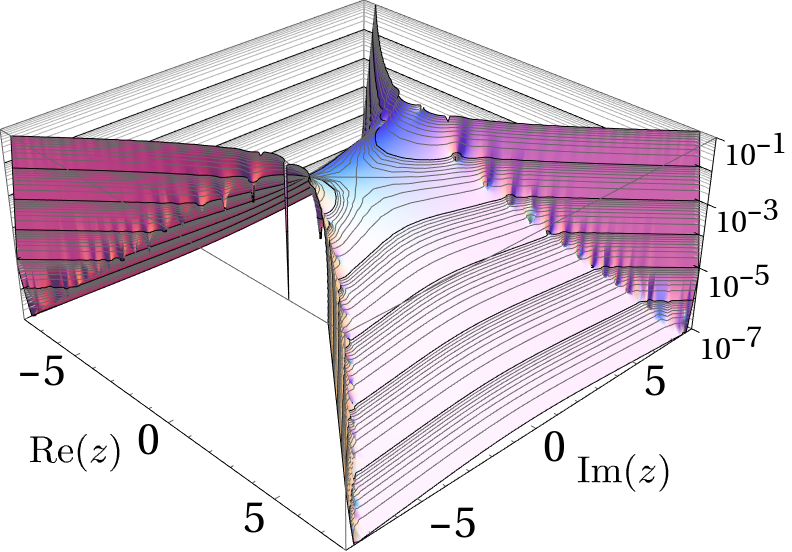
\includegraphics[scale=1]{4-Potentials/Figures/figure4Fa.png}
  }
  &
  \subfloat[$|\Vgnum(\vbr)-\Vg(\vbr)|/|\Vg(\vbr)$]{
    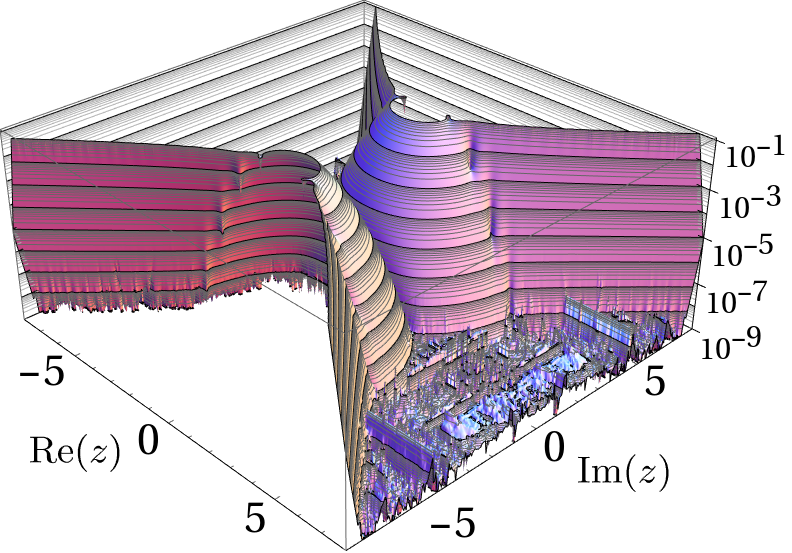
\includegraphics[scale=1]{4-Potentials/Figures/figure4Fb.png}
  }
  \end{tabular}
  \caption[Residuals between the electrostatic potentials $\Ve(\vbr)$ and $\Vg(\vbr)$, from exponential and gaussian charges, and $\Vgnum(\vbr)$ and $\Vg(\vbr)$ from numerical and exact integration for a gaussian charge, showing agreement where $\Re(\vbr^2)>0$]{
  Normalized differences between the exponential-charge potential $\Vg(\vbr)$ and the exact gaussian potential $\Vg(\vbr)$ as a reference (a), and the numerically-integrated potential $\Vgnum(\vbr)$ of section \ref{sec:quantum-chemical-potentials-complex}, against $\Vg(\vbr)$ (b), on a logarithmic scale. The plots use the same cut over complex space as Figs.~\ref{f4-numerical-potential-from-gaussian}, \ref{f4-cauchy-riemann-for-numerical-gaussian}, \ref{f4-exact-gaussian-vs-exponential-complex-coordinates} and \ref{f4-potentials-comparison-restricted-complex-coordinates} and are (roughly) restricted the allowed region $\Re(\vbr^2)>0$ of~\eqref{e4-re-r2-less-than-0}. The agreement here is not only qualitatively good, as shown in \reffig{f4-potentials-comparison-restricted-complex-coordinates}, but also quantitatively rather close, with the potentials agreeing to better than 1\% over large regions. On the other hand, once the mostly-imaginary region $\Re(\vbr^2)<0$ is reached, the disagreement rises very steeply.
  }
  \label{f4-quantitative-agreements-between-potentials}
\end{figure}




On the other hand, the close match between the potentials in the region $\Re(\vbr^2)>0$ is also a cause for concern, because it carries no warning of the wild disagreements that sprout between them with alarming speed upon leaving this region. If one is using some local method to extend the domain of the electrostatic potential, for example, how is one to detect and handle a sudden, catastrophic blow-up in the potential? It bears emphasizing that the remarkably similar surfaces shown in \reffig{f4-quantitative-agreements-between-potentials} are solutions of the \textit{same} rigid differential equation discussed in the Mathematical Aside~\ref{aside.analytical-continuation} -- a differential equation which enforces the uniqueness of its solutions over their entire domains when given (exact) agreement even at a single accumulation point -- and yet these solutions can still depart from each other, suddenly and steeply, as in \reffig{f4-exact-gaussian-vs-exponential-complex-coordinates}.


Given all of this, can we say that both $\Vg(\vbr)$ and $\Ve(\vbr)$ have the ``right'' shapes in the region where $\Re(\vbr^2)>0$, if their minute differences can lead to wildly different behaviour at a moment's notice? If it is possible to talk about a ``correct'' shape, which one is it? If both can be right depending on circumstances, which one should we use to set expectations for the physical charge density in a real-world molecule?






\section{Outlook}
In the end, unfortunately, none of these questions have any easy answers. Simply put, the theory of analytical functions is just too rigid, and depends too delicately on the initial boundary values, to say anything of consequence about the global behaviour of a general electrostatic potential $V(\vbr)$ over the entirety of complex $\vbr$ space, and the overall recommendation is to stay, whenever possible, in the `safe' region
\begin{equation}
\Re(\vbr^2)>0,
\backtag{e4-re-r2-less-than-0}
\end{equation}
where the different approaches agree.

One might also ask, at this point, for what evidence we have that the problem is even solvable: to what extent do we know that there even exists an analytical continuation for the electrostatic potential $V(\vbr)$ of a generic real-world (transition) charge density $\rho(\vbr)$? Here (regardless of whether this is fortunate or unfortunate) the answer is positive: in general, this analytical continuation does exist, at least for some open set about the real~slice of complex $\vbr$ space.


The reason for this is that the electrostatic potential $V(\vbr)$ is a solution of the Poisson equation~\eqref{e4-poisson-equation}, and it therefore gets many of its properties from the robust structure of the Laplacian operator; more specifically, the Laplacian is required to have analytic solutions whenever the right-hand side is analytic. Similarly, this right-hand-side function $\rho(\vbr)$ is obtained from the eigenfunctions of the time-independent Schrödinger equation on multiple dimensions,%
\footnote{%
This does entail a nontrivial step in showing that an analytical solution of the Schrödinger equation give an analytical charge density, since expressions of the form $\phi_m(\vbr)^* \phi_n(\vbr)$ include a complex conjugation that can destroy the analyticity if not done correctly. Fortunately, this can be done easily by extending functions of the form $\phi_m(\vbr)^*$ to the complex plane as $\phi_m(\vbr^*)^*$, which is analytic by the Schwarz reflection principle~\cite[p.~119-120]{noguchi_complex_analysis}.
}
% (admittedly through a procedure that can involve an analyticity-denying conjugation in $\phi_m(\vbr)^* \phi_n(\vbr)$, which can nevertheless be factored away as the eigenfunctions can always be chosen to be real), 
and again the Schrödinger multi-electron Hamiltonian is generally regular enough that its eigenfunctions are analytic.



\begin{mathaside}{Analytic regularity of elliptic operators}
\label{aside.elliptic-regularity}

As a final building block of the mathematics that underpins this chapter, it is also worth detailing the results that guarantee the existence of the analytical continuations of the electrostatic potentials $V(\vbr)$ that we need. The main such result is the Elliptic Regularity Theorem, which governs the regularity of solutions of elliptic partial differential equations; it can be phrased in a number of ways but a suitably strong one is provided by L. Hörmander in \citer{hormander_pdes}, p.~178, as the following theorem:

\begin{theorem}
Let $P(x, D)$ be an elliptic differential operator in $D$ with coefficients that are analytic in $D$. If $u\in \mathscr D'(\Omega)$ and 
\begin{equation}
P(x, D)u = f 
\end{equation}
where $f$ is also analytic in $\Omega$, then $u$ is analytic in $\Omega$. 
\end{theorem}


Here $\mathscr D'(\Omega)$ denotes the set of all distributions over $\Omega$ (formally defined as a set of suitably bounded linear functionals $u\colon C_0^\infty(\Omega) \to \mathbb{C}$), but the requirement that $f$ and $u$ be analytical turns them into regular functions over $\Omega$ and fulfils the boundedness condition on the distribution. %\\[-8pt]

%
%Theorems of this form, guaranteeing differentiability properties of the solution $u$ to a partial differential equation $P(x,D)u=f$ with a well-behaved right-hand side $f$, are generally known as regularity theorems, and they typically hold strictly for elliptic operators. In particular, the Elliptic Regularity Theorem guarantees a smooth solution to elliptic PDEs whenever the right-hand side is smooth, and in general operators with this property are called hypoelliptic. Similarly, the stronger requirement of analytical solutions to analytical initial data is termed analytic hypoellipticity.

\vspace{\maskip}
In particular, both the Schrödinger and the Poisson equations are of this form (once one excludes the Coulomb singularities), since they are both elliptic and have analytical coefficients and right-hand sides, so both are required to have analytical solutions.

\end{mathaside}



We have, then, the promise from an existence theorem that, given an idealized real-world (transition) charge density $\rho(\vbr)$, there should be a Platonic `true' analytical continuation of the relevant electrostatic potential $V(\vbr)$: the multi-electron Hamiltonian has analytical true eigenfunctions, which combine into an analytical charge density, and this then gives an analytical electrostatic potential. However, we have no way to find this `true' potential (which is relatively reasonable, as we cannot even find the true eigenfunctions) or even have any idea of what it should behave like, let alone find reasonable approximations for it (and this does break the usual paradigms).

One could think, for example, that to find an analytical continuation it would hopefully be good enough to find chemical data for the charge density and the electrostatic potential for real coordinates which was accurate enough, and then if necessary perform a numerical solution of the Cauchy-Riemann equations for these data. Unfortunately, such an effort is doomed to fail: the numerical solution of the Cauchy-Riemann problem is likely to prove a stiff, unstable problem, because -- as demonstrated in Figs.~\ref{f4-potentials-comparison-restricted-complex-coordinates} and \ref{f4-exact-gaussian-vs-exponential-complex-coordinates} -- very similar initial conditions can lead to very sudden, unexpected divergences, even for exactly-known potentials.

Moreover, even if we \textit{could} somehow perform this numerical solution of the Cauchy-Riemann equations to arbitrary accuracy over the entire complex plane, we would still be left with the wrong solution. This is because the quantum chemical data, in the end, produces a charge density $\rho(\vbr)$ which is ultimately a sum of gaussian-type distributions. To be sure, these will come in many places and sizes, to approximate to high accuracy the long tails and the sharp cusps of the expected real-world distribution, but in the end it will still be a finite superposition of gaussians, and the exact solution will still be the corresponding finite superposition of~$\Vg(\vbr)$s. 

Thus, it is conceivable that we could succeed in numerically solving the Cauchy-Riemann problem to accuracy close enough to the exact solution -- but we already know what this exact solution looks like: it is the relevant superposition of gaussian potentials $\Vg(\vbr)$ from \eqref{e4-exact-gaussian-potential}, and we know that these potentials diverge when $\Re(\vbr^2)<0$ as shown in~\reffig{f4-exact-gaussian-vs-exponential-complex-coordinates}, and that they do not match the exponential model which is more physically reasonable.

Similarly, one might hope that for a real molecule these divergences would cancel out in some way, but as we have seen, this is very unlikely. Instead, large $\Im(\vbr)$ any superposition-of-$\Vg(\vbr)$s potential will be dominated by the contribution from the smallest gaussians, which are typically used to approximate the cusps at the nuclei, since these will have the shortest length scales $\sigma$, and therefore their corresponding potentials $\Vg(\vbr)\sim \exp(+\Im(\vbr)^2/\sigma^2)$ will be the fastest to explode.


Even worse, the close match between $\Ve(\vbr)$ and $\Vg(\vbr)$ in the allowed region bodes ill for any finitary approach to the potential through the charge distribution. To see this, suppose that we are given a guarantee of a uniform approximation to the Platonic charge density $\rho(\vbr)$, represented as a finite sum of manageable charge densities $\rho_i(\vbr)$. This is a rather reasonable thing to assume, and it is attained, for example, when solving for $\rho(\vbr)$ through Slater-type quantum chemical methods, which offer guarantees of the form $\left|\rho(\vbr)-\sum_i\rho_i(\vbr)\right|<\eps$, where $\eps$ is a numerical precision that can be set arbitrarily small (with a corresponding increase in the size and complexity of $\sum_i\rho_i(\vbr)$), and moreover the approximation is guaranteed for \textit{all} positions $\vbr$. Even a situation this ideal, however, fails to exclude the possibility that the Platonic charge density be equal to $\rho(\vbr) = \sum_i\rho_i(\vbr) + \eps'\rho_g(\vbr)$: the manageable numerical $\sum_i\rho_i(\vbr)$, with a small gaussian addendum $\eps'\rho_g(\vbr)$ which is bounded below $\eps$ for all real positions, but which will still quickly dominate the potential at imaginary positions that are large enough.



This therefore means that, although exponential charge densities are probably the most physically correct models for the Platonic charge distribution -- the one obtained mathematically from the regularity of the Schrödinger equation --, there is still uncertainty as to how well they extend to the complex plane. 

More mathematically, this means that while analytical continuation is possible and exact when we know the exact function we want to continue analytically, the use of finitely accurate data on a limited number of sample points to attempt an analytical continuation to the whole of the complex plane is, in the absence of very strict guarantees on the function we're approximating, bound to fail at least some of the time.




We see, then, that roughly half of complex $\vbr$ space is closed to the means of inquiry we have available to us, and we need to stay in the allowed region if we want to have meaningful electrostatic potentials from our transition charges.

However, in contrast with the bleak landscape presented above, the assumption of an exponential charge is in fact fairly reasonable, and the remarkably close agreement between the potentials as displayed in \reffig{f4-potentials-comparison-restricted-complex-coordinates} is a very encouraging sign that, within the allowed region, it is actually quite reasonable to assume that we've got the correct potential, even if we're using gaussian-based quantum chemical charge distributions.

Moreover, we also have a very clean criterion -- whether $\Re(\vbr^2)>0$ or not -- to tell whether we are in the allowed region, and we can use this information to help shape the complex-space trajectory $\rl(t)$ that we will actually use to probe the potential. In addition to this clear bound, in the next chapter we will show that it is in fact possible to choose the integration path in the complex time plane in a way that keeps the position-space trajectory completely within the allowed region, and that therefore the problematic cases never arise. 

In other words, the semiclassical quantum mechanics of complex-valued trajectories need to be handled carefully, and we have seen the serious breakdowns that can occur when one pushes too far, but we can also be fairly confident that within the bounds that we have described the behaviour will be manageable, and we will show in chapter~\ref{chap:quantum-orbits} how to ensure that the trajectory remains within those bounds.


Finally, and as an added bonus, we also get that as long as we stay in the allowed region, we can safely use the exact potentials $\Vg(\vbr)$ for each of the gaussian building blocks of any quantum chemical charge distributions, and this spares us the need of any numerical integration (which was ultimately doomed to produce non-analytical results in the first place), which therefore considerably speeds up the calculations of the ARM correlation-driven ionization yield, since we now require only a few queries of the $\Vg(\vbr)$ per temporal integration point, instead of iterating over a full numerical integration.


































   